% Seminar 10: State space models, Kalman filter and Markov switching
% Time Series Analysis -- Bachelor's programmes Economic Informatics and Economic Cybernetics, Bucharest University of Economic Studies
% GENERATED by latex/build_seminar10.py -- edit the generator, not this file.
% Student version by default; the instructor version is the *_solutions.tex wrapper.
\makeatletter\@ifundefined{ifsolutions}{\expandafter\newif\csname ifsolutions\endcsname}{}\makeatother

\newcommand{\coursename}{Time Series Analysis}
% Preambul comun TSA -- Serii de timp / Time Series Analysis (Beamer, 16:9)
% Același design ca MFM și SFM (preluat din SFM, 5 octombrie 2026). Înainte de % Preambul comun TSA -- Serii de timp / Time Series Analysis (Beamer, 16:9)
% Același design ca MFM și SFM (preluat din SFM, 5 octombrie 2026). Înainte de % Preambul comun TSA -- Serii de timp / Time Series Analysis (Beamer, 16:9)
% Același design ca MFM și SFM (preluat din SFM, 5 octombrie 2026). Înainte de \input{../../latex/preamble} se definește
%   \newcommand{\coursename}{Time Series Analysis}      (EN)
%   \newcommand{\coursename}{Serii de timp}       (RO)  și  \def\tsalang{ro}
% Fișierele .tex se află în EN/Courses, EN/Seminars, RO/Cursuri, RO/Seminarii (două niveluri sub rădăcină).
% Deck-urile sînt generate de latex/build_chapterN.py / build_seminarN.py (vezi latex/tsa_build.py).

\documentclass[9pt, aspectratio=169, t]{beamer}
\providecommand{\coursename}{Time Series Analysis}

% Ensure content fits on slides
\setbeamersize{text margin left=8mm, text margin right=8mm}
% Smaller institute font (title page)
\setbeamerfont{institute}{size=\footnotesize}

%=============================================================================
% THEME AND STYLE CONFIGURATION
%=============================================================================
\usetheme{default}
% Using default theme for clean header/footer control

% Color Palette (matching Redispatch PDF)
\definecolor{MainBlue}{RGB}{26, 58, 110}
\definecolor{AccentBlue}{RGB}{26, 58, 110}
\definecolor{IDAred}{RGB}{205, 0, 0}
\definecolor{DarkGray}{RGB}{51, 51, 51}
\definecolor{MediumGray}{RGB}{128, 128, 128}
\definecolor{LightGray}{RGB}{248, 248, 248}
\definecolor{VeryLightGray}{RGB}{235, 235, 235}
\definecolor{KeynoteGray}{RGB}{218, 218, 218}
\definecolor{SectionGray}{RGB}{120, 120, 120}
\definecolor{FooterGray}{RGB}{100, 100, 100}
\definecolor{Crimson}{RGB}{220, 53, 69}
\definecolor{Forest}{RGB}{46, 125, 50}
\definecolor{Amber}{RGB}{181, 133, 63}
\definecolor{Orange}{RGB}{230, 126, 34}
\definecolor{Purple}{RGB}{142, 68, 173}

% Gradient background (exact Keynote 315° gradient: white to RGB 218,218,218)
\setbeamertemplate{background}{%
    \begin{tikzpicture}[remember picture, overlay]
        \shade[shading=axis, shading angle=315,
        top color=white, bottom color=KeynoteGray]
        (current page.south west) rectangle (current page.north east);
    \end{tikzpicture}%
}
% Fallback solid color for compatibility
\setbeamercolor{background canvas}{bg=}

\setbeamercolor{palette primary}{bg=MainBlue, fg=white}
\setbeamercolor{palette secondary}{bg=MainBlue!85, fg=white}
\setbeamercolor{palette tertiary}{bg=MainBlue!70, fg=white}
\setbeamercolor{structure}{fg=MainBlue}
\setbeamercolor{title}{fg=IDAred}
\setbeamercolor{frametitle}{fg=IDAred, bg=}
\setbeamercolor{block title}{bg=MainBlue, fg=white}
\setbeamercolor{block body}{bg=VeryLightGray, fg=DarkGray}
\setbeamercolor{block title alerted}{bg=Crimson, fg=white}
\setbeamercolor{block body alerted}{bg=Crimson!8, fg=DarkGray}
\setbeamercolor{block title example}{bg=Forest, fg=white}
\setbeamercolor{block body example}{bg=Forest!8, fg=DarkGray}
\setbeamercolor{item}{fg=MainBlue}

% Footer colors (override Madrid theme blue)
\setbeamercolor{author in head/foot}{fg=FooterGray, bg=}
\setbeamercolor{title in head/foot}{fg=FooterGray, bg=}
\setbeamercolor{date in head/foot}{fg=FooterGray, bg=}
\setbeamercolor{section in head/foot}{fg=FooterGray, bg=}
\setbeamercolor{subsection in head/foot}{fg=FooterGray, bg=}

% Bullet styles (apply everywhere including blocks)
\setbeamertemplate{itemize item}{\color{MainBlue}$\boxdot$}
\setbeamertemplate{itemize subitem}{\color{MainBlue}$\blacktriangleright$}
\setbeamertemplate{itemize subsubitem}{\color{MainBlue}\tiny$\bullet$}
\setbeamertemplate{itemize/enumerate body begin}{\normalsize}
\setbeamertemplate{itemize/enumerate subbody begin}{\normalsize}

% Item spacing - compact style
\setlength{\leftmargini}{10pt}       % Level 1: minimal indent
\setlength{\leftmarginii}{10pt}      % Level 2: minimal additional indent
% Compact list spacing (zero extra space before/after lists in blocks)
\makeatletter
\def\@listi{\leftmargin\leftmargini \topsep 0pt \parsep 0pt \itemsep 0pt}
\def\@listii{\leftmargin\leftmarginii \topsep 0pt \parsep 0pt \itemsep 0pt}
\makeatother

\setbeamertemplate{navigation symbols}{}

%=============================================================================
% CUSTOM HEADLINE
%=============================================================================
\setbeamertemplate{headline}{%
    \vskip10pt%
    \hbox to \paperwidth{%
        \hskip0.5cm%
        {\small\color{FooterGray}\renewcommand{\hyperlink}[2]{##2}\insertsectionhead}%
        \hfill%
        \textcolor{FooterGray}{\small\insertframenumber}%
        \hskip0.5cm%
    }%
    \vskip4pt%
    {\color{FooterGray}\hrule height 0.4pt}%
}

%=============================================================================
% CUSTOM FOOTER
%=============================================================================
\usepackage{fontawesome5}

\setbeamertemplate{footline}{%
    {\color{FooterGray}\hrule height 0.4pt}%
    \vskip4pt%
    \hbox to \paperwidth{%
        \hskip0.5cm%
        \textcolor{FooterGray}{\small\coursename}%
        \hfill%
        \raisebox{-0.1em}{%
            \begin{tikzpicture}[x=0.08em, y=0.08em, line width=0.4pt]
                \draw[FooterGray] (0,3) -- (1,4) -- (2,3.5) -- (3,5) -- (4,4) -- (5,6) -- (6,5.5) -- (7,4) -- (8,5) -- (9,7) -- (10,6) -- (11,5) -- (12,6.5) -- (13,8) -- (14,7) -- (15,6) -- (16,7.5) -- (17,9) -- (18,8) -- (19,7) -- (20,8.5) -- (21,10) -- (22,9) -- (23,8) -- (24,9.5);
            \end{tikzpicture}%
        }%
        \hskip0.5cm%
    }%
    \vskip6pt%
}

%=============================================================================
% PACKAGES
%=============================================================================
\usepackage[utf8]{inputenc}
\DeclareUnicodeCharacter{03B1}{\ensuremath{\alpha}}
\usepackage[T1]{fontenc}
\usepackage{amsmath, amssymb, amsthm}
\usepackage{mathtools}
\usepackage{bm}
\usepackage{tikz}
\usetikzlibrary{arrows.meta, positioning, shapes, calc, decorations.pathreplacing, shadings}
\usepackage{booktabs}
\usepackage{multirow}
\usepackage{array}
\usepackage{graphicx}
\usepackage{animate}
\usepackage{hyperref}
\usepackage{colortbl}
\usepackage{listings}
\lstset{language=Python, basicstyle=\ttfamily\scriptsize, keywordstyle=\color{MainBlue}\bfseries,
  commentstyle=\color{Forest}, stringstyle=\color{Crimson}, breaklines=true,
  frame=none, backgroundcolor=\color{VeryLightGray}, xleftmargin=2mm}
\hypersetup{colorlinks=true, linkcolor=MainBlue, urlcolor=MainBlue}
\graphicspath{{../../logos/}{../../charts/}{../../photos/}}
\usepackage{xcolor}
\hfuzz=2pt  % Suppress tiny overfull warnings (<2pt)
\vfuzz=2pt  % Suppress tiny vertical overfull warnings (<2pt)
% \mathrm in the sans-serif family of the slides (beamer resets \mathrm to the serif family at \begin{document};
% this hook runs after beamer's, so WN, Var, RMSE, ... in formulas match the surrounding text)
% Bold vectors and matrices in the same sans-serif family: \mathbf{A} in sans bold (beamer's own \mathbf came out in
% medium weight), and the bold upright Greek capitals of \boldsymbol / \bm (\bSigma, \bPhi, \boldsymbol{\Theta}) in
% cmss bold: bm.sty fixes its "boldoperators" font when it is loaded (serif cmbx), before beamer switches the
% operators to cmss, so it is reset here.
\AtBeginDocument{%
  \SetMathAlphabet{\mathrm}{normal}{\encodingdefault}{\sfdefault}{\mddefault}{n}%
  \SetMathAlphabet{\mathrm}{bold}{\encodingdefault}{\sfdefault}{bx}{n}%
  \SetMathAlphabet{\mathbf}{normal}{\encodingdefault}{\sfdefault}{bx}{n}%
  \SetMathAlphabet{\mathbf}{bold}{\encodingdefault}{\sfdefault}{bx}{n}%
  \SetSymbolFont{boldoperators}{normal}{OT1}{cmss}{bx}{n}%
  \SetSymbolFont{boldoperators}{bold}{OT1}{cmss}{bx}{n}}

%=============================================================================
% QUANTLET COMMANDS
%   \quantlet{<displayed name>}{<url>}       (generic, compatible with the older TSA decks)
%   \tsaquantlet{Ch_05}{TSA_ch5_garch}       -> https://github.com/danpele/Time-Series-Analysis/tree/main/Quantlets/Ch_05/TSA_ch5_garch
%   \qlurl{<folder>} is defined per chapter by the generator (Quantlets/Ch_NN/<folder>)
%=============================================================================
\newcommand{\tsarepo}{https://github.com/danpele/Time-Series-Analysis}
\newcommand{\tsaqlbase}{https://github.com/danpele/Time-Series-Analysis/tree/main/Quantlets}
\newcommand{\quantlet}[2]{%
    \hfill\href{#2}{%
        \raisebox{-0.15em}{
\includegraphics[height=0.7em]{ql_logo.png}}%
        \textcolor{MainBlue}{\tiny\ #1}%
    }%
}
\newcommand{\tsaquantlet}[2]{\quantlet{\detokenize{#2}}{\tsaqlbase/#1/#2}}

%=============================================================================
% NOTEBOOKS (Google Colab)
%   \colaburl{notebooks/EN/chapter5_seminar_notebook.ipynb} -> the Colab link of a file in the TSA repo
%   \nb: the chapter notebook (each seminar deck redefines it with \renewcommand)
%=============================================================================
\newcommand{\colaburl}[1]{https://colab.research.google.com/github/danpele/Time-Series-Analysis/blob/main/#1}
\newcommand{\nb}{https://colab.research.google.com/github/danpele/Time-Series-Analysis/tree/main/notebooks/EN}
\newcommand{\nbname}{notebooks/EN}

%=============================================================================
% SLIDE HELPERS (used by the generators; the same as in MFM)
%=============================================================================
% local font size for list bodies (the preamble forces \normalsize)
\newcommand{\itemsize}[1]{\setbeamertemplate{itemize/enumerate body begin}{#1}\setbeamertemplate{itemize/enumerate subbody begin}{#1}}
\newcommand{\intitle}[1]{{\hypersetup{urlcolor=white}#1}}   % white links inside coloured title bars
\newcommand{\imgcap}[1]{{\scriptsize #1}\\[0.5mm]}          % caption under a photo
\newcommand{\imgcredit}[2]{{\tiny\color{FooterGray}\href{#1}{#2}}}   % image credit: source URL, author/licence
\newcommand{\aiprompt}[1]{{\ttfamily\color{MainBlue}#1}}     % a prompt to an AI assistant

%=============================================================================
% SEMINARS: student version by default; the instructor wrapper *_solutions.tex sets \solutionstrue
%=============================================================================
\makeatletter\@ifundefined{ifsolutions}{\expandafter\newif\csname ifsolutions\endcsname}{}\makeatother
\newcommand{\solonly}[1]{\ifsolutions #1\fi}
\newcommand{\propsub}{\ifsolutions\else\framesubtitle{\ifdefined\tsalang Rezolvarea se discută la seminar\else Solution discussed in class\fi}\fi}

%=============================================================================
% APPENDIX AND CHAPTER LINKS (latex/appendix_links.py writes the calls; it also re-declares these
% macros before \begin{document}, so the decks compile with or without this preamble block)
%=============================================================================
\providecommand{\tsaapplink}[3]{\hypertarget{#2}{}\hyperlink{#1}{\beamergotobutton{#3}}}
\providecommand{\tsaappback}[2]{\begin{tikzpicture}[remember picture,overlay]\node[anchor=south east] at ([xshift=-3mm,yshift=7mm]current page.south east){\hyperlink{#1}{\beamerreturnbutton{#2}}};\end{tikzpicture}}
\providecommand{\tsachlink}[2]{\href{#1}{#2}}
\providecommand{\tsachlinkt}[2]{\href{#1}{\usebeamercolor[fg]{frametitle}#2}}

%=============================================================================
% QUANTINAR COMMAND: link către un curs Quantinar (subiecte avansate)
%=============================================================================
\newcommand{\quantinar}[2]{%
    \href{#2}{%
        \raisebox{-0.15em}{
\includegraphics[height=0.8em]{qr_logo.png}}%
        \textcolor{MainBlue}{\scriptsize\ #1}%
    }%
}

%=============================================================================
% CUSTOM TITLE PAGE
%=============================================================================
\defbeamertemplate*{title page}{hybrid}[1][]
{
    \vspace{0.2cm}
    % Logos row - top header (with clickable links)
    \begin{center}
        \href{https://www.ase.ro}{
\includegraphics[height=1.0cm]{ase_logo.png}}\hspace{0.3cm}%
        \href{https://theida.net}{
\includegraphics[height=1.0cm]{ida_logo.png}}\hspace{0.3cm}%
        \href{https://blockchain-research-center.com}{
\includegraphics[height=1.0cm]{brc_logo.png}}\hspace{0.3cm}%
        \href{https://www.ai4efin.ase.ro}{
\includegraphics[height=1.0cm]{ai4efin_logo.png}}\hspace{0.3cm}%
        \href{https://ipe.ro/new}{
\includegraphics[height=1.0cm]{acad_logo.png}}\hspace{0.3cm}%
        \href{https://www.digital-finance-msca.com}{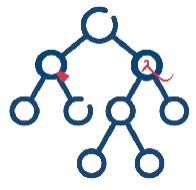
\includegraphics[height=1.0cm]{msca_logo.png}}%
    \end{center}

    \vspace{0.6cm}

    % Main title with Q logos on sides (with clickable links)
    \begin{center}
        \begin{minipage}{0.1\textwidth}
            \centering
            \href{https://quantlet.com}{
\includegraphics[height=1.1cm]{ql_logo.png}}
        \end{minipage}%
        \begin{minipage}{0.78\textwidth}
            \centering
            {\LARGE\bfseries\usebeamercolor[fg]{title}\inserttitle}

            \vspace{0.3cm}

            {\usebeamerfont{subtitle}\usebeamercolor[fg]{title}\insertsubtitle}
        \end{minipage}%
        \begin{minipage}{0.1\textwidth}
            \centering
            \href{https://quantinar.com}{
\includegraphics[height=1.1cm]{qr_logo.png}}
        \end{minipage}
    \end{center}

    \vspace{0.6cm}

    % Authors (left aligned)
    \hspace{0.5cm}{\usebeamerfont{author}\insertauthor}

    \vspace{0.3cm}

    % Institute/Affiliations (left aligned)
    \hspace{0.5cm}\begin{minipage}[t]{0.9\textwidth}
        \raggedright\small\insertinstitute
    \end{minipage}
}

%=============================================================================
% THEOREM ENVIRONMENTS
%=============================================================================
\theoremstyle{definition}
\setbeamertemplate{theorems}[numbered]
\ifdefined\tsalang
\newtheorem{defn}{Definiție}
\newtheorem{thm}{Teoremă}
\newtheorem{prop}{Propoziție}
\newtheorem{rmk}{Observație}
\else
\newtheorem{defn}{Definition}
\newtheorem{thm}{Theorem}
\newtheorem{prop}{Proposition}
\newtheorem{rmk}{Remark}
\fi

%=============================================================================
% CENTRED MINIPAGE (no extra vertical space)
%=============================================================================
\newenvironment{cminipage}[1]{%
    \par\noindent\hfill\begin{minipage}{#1}\ignorespaces
}{%
    \end{minipage}\hfill\null\par
}

%=============================================================================
% CUSTOM COMMANDS
%=============================================================================
\newcommand{\E}{\mathbb{E}}
\newcommand{\Var}{\text{Var}}
\newcommand{\Cov}{\text{Cov}}
\newcommand{\Corr}{\text{Corr}}
\newcommand{\R}{\mathbb{R}}
\newcommand{\N}{\mathbb{N}}
\newcommand{\Z}{\mathbb{Z}}
\newcommand{\B}{\mathbf{B}}
\newcommand{\imark}{\textcolor{MainBlue}{\textbullet}}
\newcommand{\RMSE}{\text{RMSE}}
\newcommand{\MAE}{\text{MAE}}
\newcommand{\MAPE}{\text{MAPE}}

% Boldface vector/matrix commands (VAR, VECM, state space; also used by the older TSA decks)
\newcommand{\bY}{\mathbf{Y}}
\newcommand{\bX}{\mathbf{X}}
\newcommand{\bA}{\mathbf{A}}
\newcommand{\bB}{\mathbf{B}}
\newcommand{\bepsilon}{\boldsymbol{\varepsilon}}
\newcommand{\bSigma}{\boldsymbol{\Sigma}}
\newcommand{\bPhi}{\boldsymbol{\Phi}}
\newcommand{\bGamma}{\boldsymbol{\Gamma}}
\newcommand{\bPi}{\boldsymbol{\Pi}}
\newcommand{\bc}{\mathbf{c}}
\newcommand{\balpha}{\boldsymbol{\alpha}}
\newcommand{\bbeta}{\boldsymbol{\beta}}
\newcommand{\bvarepsilon}{\boldsymbol{\varepsilon}}

% Legacy seminar marks (older TSA seminar decks)
\newcommand{\correct}{\textcolor{Forest}{\checkmark}}
\newcommand{\incorrect}{\textcolor{Crimson}{\texttimes}}
 se definește
%   \newcommand{\coursename}{Time Series Analysis}      (EN)
%   \newcommand{\coursename}{Serii de timp}       (RO)  și  \def\tsalang{ro}
% Fișierele .tex se află în EN/Courses, EN/Seminars, RO/Cursuri, RO/Seminarii (două niveluri sub rădăcină).
% Deck-urile sînt generate de latex/build_chapterN.py / build_seminarN.py (vezi latex/tsa_build.py).

\documentclass[9pt, aspectratio=169, t]{beamer}
\providecommand{\coursename}{Time Series Analysis}

% Ensure content fits on slides
\setbeamersize{text margin left=8mm, text margin right=8mm}
% Smaller institute font (title page)
\setbeamerfont{institute}{size=\footnotesize}

%=============================================================================
% THEME AND STYLE CONFIGURATION
%=============================================================================
\usetheme{default}
% Using default theme for clean header/footer control

% Color Palette (matching Redispatch PDF)
\definecolor{MainBlue}{RGB}{26, 58, 110}
\definecolor{AccentBlue}{RGB}{26, 58, 110}
\definecolor{IDAred}{RGB}{205, 0, 0}
\definecolor{DarkGray}{RGB}{51, 51, 51}
\definecolor{MediumGray}{RGB}{128, 128, 128}
\definecolor{LightGray}{RGB}{248, 248, 248}
\definecolor{VeryLightGray}{RGB}{235, 235, 235}
\definecolor{KeynoteGray}{RGB}{218, 218, 218}
\definecolor{SectionGray}{RGB}{120, 120, 120}
\definecolor{FooterGray}{RGB}{100, 100, 100}
\definecolor{Crimson}{RGB}{220, 53, 69}
\definecolor{Forest}{RGB}{46, 125, 50}
\definecolor{Amber}{RGB}{181, 133, 63}
\definecolor{Orange}{RGB}{230, 126, 34}
\definecolor{Purple}{RGB}{142, 68, 173}

% Gradient background (exact Keynote 315° gradient: white to RGB 218,218,218)
\setbeamertemplate{background}{%
    \begin{tikzpicture}[remember picture, overlay]
        \shade[shading=axis, shading angle=315,
        top color=white, bottom color=KeynoteGray]
        (current page.south west) rectangle (current page.north east);
    \end{tikzpicture}%
}
% Fallback solid color for compatibility
\setbeamercolor{background canvas}{bg=}

\setbeamercolor{palette primary}{bg=MainBlue, fg=white}
\setbeamercolor{palette secondary}{bg=MainBlue!85, fg=white}
\setbeamercolor{palette tertiary}{bg=MainBlue!70, fg=white}
\setbeamercolor{structure}{fg=MainBlue}
\setbeamercolor{title}{fg=IDAred}
\setbeamercolor{frametitle}{fg=IDAred, bg=}
\setbeamercolor{block title}{bg=MainBlue, fg=white}
\setbeamercolor{block body}{bg=VeryLightGray, fg=DarkGray}
\setbeamercolor{block title alerted}{bg=Crimson, fg=white}
\setbeamercolor{block body alerted}{bg=Crimson!8, fg=DarkGray}
\setbeamercolor{block title example}{bg=Forest, fg=white}
\setbeamercolor{block body example}{bg=Forest!8, fg=DarkGray}
\setbeamercolor{item}{fg=MainBlue}

% Footer colors (override Madrid theme blue)
\setbeamercolor{author in head/foot}{fg=FooterGray, bg=}
\setbeamercolor{title in head/foot}{fg=FooterGray, bg=}
\setbeamercolor{date in head/foot}{fg=FooterGray, bg=}
\setbeamercolor{section in head/foot}{fg=FooterGray, bg=}
\setbeamercolor{subsection in head/foot}{fg=FooterGray, bg=}

% Bullet styles (apply everywhere including blocks)
\setbeamertemplate{itemize item}{\color{MainBlue}$\boxdot$}
\setbeamertemplate{itemize subitem}{\color{MainBlue}$\blacktriangleright$}
\setbeamertemplate{itemize subsubitem}{\color{MainBlue}\tiny$\bullet$}
\setbeamertemplate{itemize/enumerate body begin}{\normalsize}
\setbeamertemplate{itemize/enumerate subbody begin}{\normalsize}

% Item spacing - compact style
\setlength{\leftmargini}{10pt}       % Level 1: minimal indent
\setlength{\leftmarginii}{10pt}      % Level 2: minimal additional indent
% Compact list spacing (zero extra space before/after lists in blocks)
\makeatletter
\def\@listi{\leftmargin\leftmargini \topsep 0pt \parsep 0pt \itemsep 0pt}
\def\@listii{\leftmargin\leftmarginii \topsep 0pt \parsep 0pt \itemsep 0pt}
\makeatother

\setbeamertemplate{navigation symbols}{}

%=============================================================================
% CUSTOM HEADLINE
%=============================================================================
\setbeamertemplate{headline}{%
    \vskip10pt%
    \hbox to \paperwidth{%
        \hskip0.5cm%
        {\small\color{FooterGray}\renewcommand{\hyperlink}[2]{##2}\insertsectionhead}%
        \hfill%
        \textcolor{FooterGray}{\small\insertframenumber}%
        \hskip0.5cm%
    }%
    \vskip4pt%
    {\color{FooterGray}\hrule height 0.4pt}%
}

%=============================================================================
% CUSTOM FOOTER
%=============================================================================
\usepackage{fontawesome5}

\setbeamertemplate{footline}{%
    {\color{FooterGray}\hrule height 0.4pt}%
    \vskip4pt%
    \hbox to \paperwidth{%
        \hskip0.5cm%
        \textcolor{FooterGray}{\small\coursename}%
        \hfill%
        \raisebox{-0.1em}{%
            \begin{tikzpicture}[x=0.08em, y=0.08em, line width=0.4pt]
                \draw[FooterGray] (0,3) -- (1,4) -- (2,3.5) -- (3,5) -- (4,4) -- (5,6) -- (6,5.5) -- (7,4) -- (8,5) -- (9,7) -- (10,6) -- (11,5) -- (12,6.5) -- (13,8) -- (14,7) -- (15,6) -- (16,7.5) -- (17,9) -- (18,8) -- (19,7) -- (20,8.5) -- (21,10) -- (22,9) -- (23,8) -- (24,9.5);
            \end{tikzpicture}%
        }%
        \hskip0.5cm%
    }%
    \vskip6pt%
}

%=============================================================================
% PACKAGES
%=============================================================================
\usepackage[utf8]{inputenc}
\DeclareUnicodeCharacter{03B1}{\ensuremath{\alpha}}
\usepackage[T1]{fontenc}
\usepackage{amsmath, amssymb, amsthm}
\usepackage{mathtools}
\usepackage{bm}
\usepackage{tikz}
\usetikzlibrary{arrows.meta, positioning, shapes, calc, decorations.pathreplacing, shadings}
\usepackage{booktabs}
\usepackage{multirow}
\usepackage{array}
\usepackage{graphicx}
\usepackage{animate}
\usepackage{hyperref}
\usepackage{colortbl}
\usepackage{listings}
\lstset{language=Python, basicstyle=\ttfamily\scriptsize, keywordstyle=\color{MainBlue}\bfseries,
  commentstyle=\color{Forest}, stringstyle=\color{Crimson}, breaklines=true,
  frame=none, backgroundcolor=\color{VeryLightGray}, xleftmargin=2mm}
\hypersetup{colorlinks=true, linkcolor=MainBlue, urlcolor=MainBlue}
\graphicspath{{../../logos/}{../../charts/}{../../photos/}}
\usepackage{xcolor}
\hfuzz=2pt  % Suppress tiny overfull warnings (<2pt)
\vfuzz=2pt  % Suppress tiny vertical overfull warnings (<2pt)
% \mathrm in the sans-serif family of the slides (beamer resets \mathrm to the serif family at \begin{document};
% this hook runs after beamer's, so WN, Var, RMSE, ... in formulas match the surrounding text)
% Bold vectors and matrices in the same sans-serif family: \mathbf{A} in sans bold (beamer's own \mathbf came out in
% medium weight), and the bold upright Greek capitals of \boldsymbol / \bm (\bSigma, \bPhi, \boldsymbol{\Theta}) in
% cmss bold: bm.sty fixes its "boldoperators" font when it is loaded (serif cmbx), before beamer switches the
% operators to cmss, so it is reset here.
\AtBeginDocument{%
  \SetMathAlphabet{\mathrm}{normal}{\encodingdefault}{\sfdefault}{\mddefault}{n}%
  \SetMathAlphabet{\mathrm}{bold}{\encodingdefault}{\sfdefault}{bx}{n}%
  \SetMathAlphabet{\mathbf}{normal}{\encodingdefault}{\sfdefault}{bx}{n}%
  \SetMathAlphabet{\mathbf}{bold}{\encodingdefault}{\sfdefault}{bx}{n}%
  \SetSymbolFont{boldoperators}{normal}{OT1}{cmss}{bx}{n}%
  \SetSymbolFont{boldoperators}{bold}{OT1}{cmss}{bx}{n}}

%=============================================================================
% QUANTLET COMMANDS
%   \quantlet{<displayed name>}{<url>}       (generic, compatible with the older TSA decks)
%   \tsaquantlet{Ch_05}{TSA_ch5_garch}       -> https://github.com/danpele/Time-Series-Analysis/tree/main/Quantlets/Ch_05/TSA_ch5_garch
%   \qlurl{<folder>} is defined per chapter by the generator (Quantlets/Ch_NN/<folder>)
%=============================================================================
\newcommand{\tsarepo}{https://github.com/danpele/Time-Series-Analysis}
\newcommand{\tsaqlbase}{https://github.com/danpele/Time-Series-Analysis/tree/main/Quantlets}
\newcommand{\quantlet}[2]{%
    \hfill\href{#2}{%
        \raisebox{-0.15em}{
\includegraphics[height=0.7em]{ql_logo.png}}%
        \textcolor{MainBlue}{\tiny\ #1}%
    }%
}
\newcommand{\tsaquantlet}[2]{\quantlet{\detokenize{#2}}{\tsaqlbase/#1/#2}}

%=============================================================================
% NOTEBOOKS (Google Colab)
%   \colaburl{notebooks/EN/chapter5_seminar_notebook.ipynb} -> the Colab link of a file in the TSA repo
%   \nb: the chapter notebook (each seminar deck redefines it with \renewcommand)
%=============================================================================
\newcommand{\colaburl}[1]{https://colab.research.google.com/github/danpele/Time-Series-Analysis/blob/main/#1}
\newcommand{\nb}{https://colab.research.google.com/github/danpele/Time-Series-Analysis/tree/main/notebooks/EN}
\newcommand{\nbname}{notebooks/EN}

%=============================================================================
% SLIDE HELPERS (used by the generators; the same as in MFM)
%=============================================================================
% local font size for list bodies (the preamble forces \normalsize)
\newcommand{\itemsize}[1]{\setbeamertemplate{itemize/enumerate body begin}{#1}\setbeamertemplate{itemize/enumerate subbody begin}{#1}}
\newcommand{\intitle}[1]{{\hypersetup{urlcolor=white}#1}}   % white links inside coloured title bars
\newcommand{\imgcap}[1]{{\scriptsize #1}\\[0.5mm]}          % caption under a photo
\newcommand{\imgcredit}[2]{{\tiny\color{FooterGray}\href{#1}{#2}}}   % image credit: source URL, author/licence
\newcommand{\aiprompt}[1]{{\ttfamily\color{MainBlue}#1}}     % a prompt to an AI assistant

%=============================================================================
% SEMINARS: student version by default; the instructor wrapper *_solutions.tex sets \solutionstrue
%=============================================================================
\makeatletter\@ifundefined{ifsolutions}{\expandafter\newif\csname ifsolutions\endcsname}{}\makeatother
\newcommand{\solonly}[1]{\ifsolutions #1\fi}
\newcommand{\propsub}{\ifsolutions\else\framesubtitle{\ifdefined\tsalang Rezolvarea se discută la seminar\else Solution discussed in class\fi}\fi}

%=============================================================================
% APPENDIX AND CHAPTER LINKS (latex/appendix_links.py writes the calls; it also re-declares these
% macros before \begin{document}, so the decks compile with or without this preamble block)
%=============================================================================
\providecommand{\tsaapplink}[3]{\hypertarget{#2}{}\hyperlink{#1}{\beamergotobutton{#3}}}
\providecommand{\tsaappback}[2]{\begin{tikzpicture}[remember picture,overlay]\node[anchor=south east] at ([xshift=-3mm,yshift=7mm]current page.south east){\hyperlink{#1}{\beamerreturnbutton{#2}}};\end{tikzpicture}}
\providecommand{\tsachlink}[2]{\href{#1}{#2}}
\providecommand{\tsachlinkt}[2]{\href{#1}{\usebeamercolor[fg]{frametitle}#2}}

%=============================================================================
% QUANTINAR COMMAND: link către un curs Quantinar (subiecte avansate)
%=============================================================================
\newcommand{\quantinar}[2]{%
    \href{#2}{%
        \raisebox{-0.15em}{
\includegraphics[height=0.8em]{qr_logo.png}}%
        \textcolor{MainBlue}{\scriptsize\ #1}%
    }%
}

%=============================================================================
% CUSTOM TITLE PAGE
%=============================================================================
\defbeamertemplate*{title page}{hybrid}[1][]
{
    \vspace{0.2cm}
    % Logos row - top header (with clickable links)
    \begin{center}
        \href{https://www.ase.ro}{
\includegraphics[height=1.0cm]{ase_logo.png}}\hspace{0.3cm}%
        \href{https://theida.net}{
\includegraphics[height=1.0cm]{ida_logo.png}}\hspace{0.3cm}%
        \href{https://blockchain-research-center.com}{
\includegraphics[height=1.0cm]{brc_logo.png}}\hspace{0.3cm}%
        \href{https://www.ai4efin.ase.ro}{
\includegraphics[height=1.0cm]{ai4efin_logo.png}}\hspace{0.3cm}%
        \href{https://ipe.ro/new}{
\includegraphics[height=1.0cm]{acad_logo.png}}\hspace{0.3cm}%
        \href{https://www.digital-finance-msca.com}{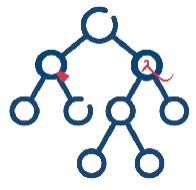
\includegraphics[height=1.0cm]{msca_logo.png}}%
    \end{center}

    \vspace{0.6cm}

    % Main title with Q logos on sides (with clickable links)
    \begin{center}
        \begin{minipage}{0.1\textwidth}
            \centering
            \href{https://quantlet.com}{
\includegraphics[height=1.1cm]{ql_logo.png}}
        \end{minipage}%
        \begin{minipage}{0.78\textwidth}
            \centering
            {\LARGE\bfseries\usebeamercolor[fg]{title}\inserttitle}

            \vspace{0.3cm}

            {\usebeamerfont{subtitle}\usebeamercolor[fg]{title}\insertsubtitle}
        \end{minipage}%
        \begin{minipage}{0.1\textwidth}
            \centering
            \href{https://quantinar.com}{
\includegraphics[height=1.1cm]{qr_logo.png}}
        \end{minipage}
    \end{center}

    \vspace{0.6cm}

    % Authors (left aligned)
    \hspace{0.5cm}{\usebeamerfont{author}\insertauthor}

    \vspace{0.3cm}

    % Institute/Affiliations (left aligned)
    \hspace{0.5cm}\begin{minipage}[t]{0.9\textwidth}
        \raggedright\small\insertinstitute
    \end{minipage}
}

%=============================================================================
% THEOREM ENVIRONMENTS
%=============================================================================
\theoremstyle{definition}
\setbeamertemplate{theorems}[numbered]
\ifdefined\tsalang
\newtheorem{defn}{Definiție}
\newtheorem{thm}{Teoremă}
\newtheorem{prop}{Propoziție}
\newtheorem{rmk}{Observație}
\else
\newtheorem{defn}{Definition}
\newtheorem{thm}{Theorem}
\newtheorem{prop}{Proposition}
\newtheorem{rmk}{Remark}
\fi

%=============================================================================
% CENTRED MINIPAGE (no extra vertical space)
%=============================================================================
\newenvironment{cminipage}[1]{%
    \par\noindent\hfill\begin{minipage}{#1}\ignorespaces
}{%
    \end{minipage}\hfill\null\par
}

%=============================================================================
% CUSTOM COMMANDS
%=============================================================================
\newcommand{\E}{\mathbb{E}}
\newcommand{\Var}{\text{Var}}
\newcommand{\Cov}{\text{Cov}}
\newcommand{\Corr}{\text{Corr}}
\newcommand{\R}{\mathbb{R}}
\newcommand{\N}{\mathbb{N}}
\newcommand{\Z}{\mathbb{Z}}
\newcommand{\B}{\mathbf{B}}
\newcommand{\imark}{\textcolor{MainBlue}{\textbullet}}
\newcommand{\RMSE}{\text{RMSE}}
\newcommand{\MAE}{\text{MAE}}
\newcommand{\MAPE}{\text{MAPE}}

% Boldface vector/matrix commands (VAR, VECM, state space; also used by the older TSA decks)
\newcommand{\bY}{\mathbf{Y}}
\newcommand{\bX}{\mathbf{X}}
\newcommand{\bA}{\mathbf{A}}
\newcommand{\bB}{\mathbf{B}}
\newcommand{\bepsilon}{\boldsymbol{\varepsilon}}
\newcommand{\bSigma}{\boldsymbol{\Sigma}}
\newcommand{\bPhi}{\boldsymbol{\Phi}}
\newcommand{\bGamma}{\boldsymbol{\Gamma}}
\newcommand{\bPi}{\boldsymbol{\Pi}}
\newcommand{\bc}{\mathbf{c}}
\newcommand{\balpha}{\boldsymbol{\alpha}}
\newcommand{\bbeta}{\boldsymbol{\beta}}
\newcommand{\bvarepsilon}{\boldsymbol{\varepsilon}}

% Legacy seminar marks (older TSA seminar decks)
\newcommand{\correct}{\textcolor{Forest}{\checkmark}}
\newcommand{\incorrect}{\textcolor{Crimson}{\texttimes}}
 se definește
%   \newcommand{\coursename}{Time Series Analysis}      (EN)
%   \newcommand{\coursename}{Serii de timp}       (RO)  și  \def\tsalang{ro}
% Fișierele .tex se află în EN/Courses, EN/Seminars, RO/Cursuri, RO/Seminarii (două niveluri sub rădăcină).
% Deck-urile sînt generate de latex/build_chapterN.py / build_seminarN.py (vezi latex/tsa_build.py).

\documentclass[9pt, aspectratio=169, t]{beamer}
\providecommand{\coursename}{Time Series Analysis}

% Ensure content fits on slides
\setbeamersize{text margin left=8mm, text margin right=8mm}
% Smaller institute font (title page)
\setbeamerfont{institute}{size=\footnotesize}

%=============================================================================
% THEME AND STYLE CONFIGURATION
%=============================================================================
\usetheme{default}
% Using default theme for clean header/footer control

% Color Palette (matching Redispatch PDF)
\definecolor{MainBlue}{RGB}{26, 58, 110}
\definecolor{AccentBlue}{RGB}{26, 58, 110}
\definecolor{IDAred}{RGB}{205, 0, 0}
\definecolor{DarkGray}{RGB}{51, 51, 51}
\definecolor{MediumGray}{RGB}{128, 128, 128}
\definecolor{LightGray}{RGB}{248, 248, 248}
\definecolor{VeryLightGray}{RGB}{235, 235, 235}
\definecolor{KeynoteGray}{RGB}{218, 218, 218}
\definecolor{SectionGray}{RGB}{120, 120, 120}
\definecolor{FooterGray}{RGB}{100, 100, 100}
\definecolor{Crimson}{RGB}{220, 53, 69}
\definecolor{Forest}{RGB}{46, 125, 50}
\definecolor{Amber}{RGB}{181, 133, 63}
\definecolor{Orange}{RGB}{230, 126, 34}
\definecolor{Purple}{RGB}{142, 68, 173}

% Gradient background (exact Keynote 315° gradient: white to RGB 218,218,218)
\setbeamertemplate{background}{%
    \begin{tikzpicture}[remember picture, overlay]
        \shade[shading=axis, shading angle=315,
        top color=white, bottom color=KeynoteGray]
        (current page.south west) rectangle (current page.north east);
    \end{tikzpicture}%
}
% Fallback solid color for compatibility
\setbeamercolor{background canvas}{bg=}

\setbeamercolor{palette primary}{bg=MainBlue, fg=white}
\setbeamercolor{palette secondary}{bg=MainBlue!85, fg=white}
\setbeamercolor{palette tertiary}{bg=MainBlue!70, fg=white}
\setbeamercolor{structure}{fg=MainBlue}
\setbeamercolor{title}{fg=IDAred}
\setbeamercolor{frametitle}{fg=IDAred, bg=}
\setbeamercolor{block title}{bg=MainBlue, fg=white}
\setbeamercolor{block body}{bg=VeryLightGray, fg=DarkGray}
\setbeamercolor{block title alerted}{bg=Crimson, fg=white}
\setbeamercolor{block body alerted}{bg=Crimson!8, fg=DarkGray}
\setbeamercolor{block title example}{bg=Forest, fg=white}
\setbeamercolor{block body example}{bg=Forest!8, fg=DarkGray}
\setbeamercolor{item}{fg=MainBlue}

% Footer colors (override Madrid theme blue)
\setbeamercolor{author in head/foot}{fg=FooterGray, bg=}
\setbeamercolor{title in head/foot}{fg=FooterGray, bg=}
\setbeamercolor{date in head/foot}{fg=FooterGray, bg=}
\setbeamercolor{section in head/foot}{fg=FooterGray, bg=}
\setbeamercolor{subsection in head/foot}{fg=FooterGray, bg=}

% Bullet styles (apply everywhere including blocks)
\setbeamertemplate{itemize item}{\color{MainBlue}$\boxdot$}
\setbeamertemplate{itemize subitem}{\color{MainBlue}$\blacktriangleright$}
\setbeamertemplate{itemize subsubitem}{\color{MainBlue}\tiny$\bullet$}
\setbeamertemplate{itemize/enumerate body begin}{\normalsize}
\setbeamertemplate{itemize/enumerate subbody begin}{\normalsize}

% Item spacing - compact style
\setlength{\leftmargini}{10pt}       % Level 1: minimal indent
\setlength{\leftmarginii}{10pt}      % Level 2: minimal additional indent
% Compact list spacing (zero extra space before/after lists in blocks)
\makeatletter
\def\@listi{\leftmargin\leftmargini \topsep 0pt \parsep 0pt \itemsep 0pt}
\def\@listii{\leftmargin\leftmarginii \topsep 0pt \parsep 0pt \itemsep 0pt}
\makeatother

\setbeamertemplate{navigation symbols}{}

%=============================================================================
% CUSTOM HEADLINE
%=============================================================================
\setbeamertemplate{headline}{%
    \vskip10pt%
    \hbox to \paperwidth{%
        \hskip0.5cm%
        {\small\color{FooterGray}\renewcommand{\hyperlink}[2]{##2}\insertsectionhead}%
        \hfill%
        \textcolor{FooterGray}{\small\insertframenumber}%
        \hskip0.5cm%
    }%
    \vskip4pt%
    {\color{FooterGray}\hrule height 0.4pt}%
}

%=============================================================================
% CUSTOM FOOTER
%=============================================================================
\usepackage{fontawesome5}

\setbeamertemplate{footline}{%
    {\color{FooterGray}\hrule height 0.4pt}%
    \vskip4pt%
    \hbox to \paperwidth{%
        \hskip0.5cm%
        \textcolor{FooterGray}{\small\coursename}%
        \hfill%
        \raisebox{-0.1em}{%
            \begin{tikzpicture}[x=0.08em, y=0.08em, line width=0.4pt]
                \draw[FooterGray] (0,3) -- (1,4) -- (2,3.5) -- (3,5) -- (4,4) -- (5,6) -- (6,5.5) -- (7,4) -- (8,5) -- (9,7) -- (10,6) -- (11,5) -- (12,6.5) -- (13,8) -- (14,7) -- (15,6) -- (16,7.5) -- (17,9) -- (18,8) -- (19,7) -- (20,8.5) -- (21,10) -- (22,9) -- (23,8) -- (24,9.5);
            \end{tikzpicture}%
        }%
        \hskip0.5cm%
    }%
    \vskip6pt%
}

%=============================================================================
% PACKAGES
%=============================================================================
\usepackage[utf8]{inputenc}
\DeclareUnicodeCharacter{03B1}{\ensuremath{\alpha}}
\usepackage[T1]{fontenc}
\usepackage{amsmath, amssymb, amsthm}
\usepackage{mathtools}
\usepackage{bm}
\usepackage{tikz}
\usetikzlibrary{arrows.meta, positioning, shapes, calc, decorations.pathreplacing, shadings}
\usepackage{booktabs}
\usepackage{multirow}
\usepackage{array}
\usepackage{graphicx}
\usepackage{animate}
\usepackage{hyperref}
\usepackage{colortbl}
\usepackage{listings}
\lstset{language=Python, basicstyle=\ttfamily\scriptsize, keywordstyle=\color{MainBlue}\bfseries,
  commentstyle=\color{Forest}, stringstyle=\color{Crimson}, breaklines=true,
  frame=none, backgroundcolor=\color{VeryLightGray}, xleftmargin=2mm}
\hypersetup{colorlinks=true, linkcolor=MainBlue, urlcolor=MainBlue}
\graphicspath{{../../logos/}{../../charts/}{../../photos/}}
\usepackage{xcolor}
\hfuzz=2pt  % Suppress tiny overfull warnings (<2pt)
\vfuzz=2pt  % Suppress tiny vertical overfull warnings (<2pt)
% \mathrm in the sans-serif family of the slides (beamer resets \mathrm to the serif family at \begin{document};
% this hook runs after beamer's, so WN, Var, RMSE, ... in formulas match the surrounding text)
% Bold vectors and matrices in the same sans-serif family: \mathbf{A} in sans bold (beamer's own \mathbf came out in
% medium weight), and the bold upright Greek capitals of \boldsymbol / \bm (\bSigma, \bPhi, \boldsymbol{\Theta}) in
% cmss bold: bm.sty fixes its "boldoperators" font when it is loaded (serif cmbx), before beamer switches the
% operators to cmss, so it is reset here.
\AtBeginDocument{%
  \SetMathAlphabet{\mathrm}{normal}{\encodingdefault}{\sfdefault}{\mddefault}{n}%
  \SetMathAlphabet{\mathrm}{bold}{\encodingdefault}{\sfdefault}{bx}{n}%
  \SetMathAlphabet{\mathbf}{normal}{\encodingdefault}{\sfdefault}{bx}{n}%
  \SetMathAlphabet{\mathbf}{bold}{\encodingdefault}{\sfdefault}{bx}{n}%
  \SetSymbolFont{boldoperators}{normal}{OT1}{cmss}{bx}{n}%
  \SetSymbolFont{boldoperators}{bold}{OT1}{cmss}{bx}{n}}

%=============================================================================
% QUANTLET COMMANDS
%   \quantlet{<displayed name>}{<url>}       (generic, compatible with the older TSA decks)
%   \tsaquantlet{Ch_05}{TSA_ch5_garch}       -> https://github.com/danpele/Time-Series-Analysis/tree/main/Quantlets/Ch_05/TSA_ch5_garch
%   \qlurl{<folder>} is defined per chapter by the generator (Quantlets/Ch_NN/<folder>)
%=============================================================================
\newcommand{\tsarepo}{https://github.com/danpele/Time-Series-Analysis}
\newcommand{\tsaqlbase}{https://github.com/danpele/Time-Series-Analysis/tree/main/Quantlets}
\newcommand{\quantlet}[2]{%
    \hfill\href{#2}{%
        \raisebox{-0.15em}{
\includegraphics[height=0.7em]{ql_logo.png}}%
        \textcolor{MainBlue}{\tiny\ #1}%
    }%
}
\newcommand{\tsaquantlet}[2]{\quantlet{\detokenize{#2}}{\tsaqlbase/#1/#2}}

%=============================================================================
% NOTEBOOKS (Google Colab)
%   \colaburl{notebooks/EN/chapter5_seminar_notebook.ipynb} -> the Colab link of a file in the TSA repo
%   \nb: the chapter notebook (each seminar deck redefines it with \renewcommand)
%=============================================================================
\newcommand{\colaburl}[1]{https://colab.research.google.com/github/danpele/Time-Series-Analysis/blob/main/#1}
\newcommand{\nb}{https://colab.research.google.com/github/danpele/Time-Series-Analysis/tree/main/notebooks/EN}
\newcommand{\nbname}{notebooks/EN}

%=============================================================================
% SLIDE HELPERS (used by the generators; the same as in MFM)
%=============================================================================
% local font size for list bodies (the preamble forces \normalsize)
\newcommand{\itemsize}[1]{\setbeamertemplate{itemize/enumerate body begin}{#1}\setbeamertemplate{itemize/enumerate subbody begin}{#1}}
\newcommand{\intitle}[1]{{\hypersetup{urlcolor=white}#1}}   % white links inside coloured title bars
\newcommand{\imgcap}[1]{{\scriptsize #1}\\[0.5mm]}          % caption under a photo
\newcommand{\imgcredit}[2]{{\tiny\color{FooterGray}\href{#1}{#2}}}   % image credit: source URL, author/licence
\newcommand{\aiprompt}[1]{{\ttfamily\color{MainBlue}#1}}     % a prompt to an AI assistant

%=============================================================================
% SEMINARS: student version by default; the instructor wrapper *_solutions.tex sets \solutionstrue
%=============================================================================
\makeatletter\@ifundefined{ifsolutions}{\expandafter\newif\csname ifsolutions\endcsname}{}\makeatother
\newcommand{\solonly}[1]{\ifsolutions #1\fi}
\newcommand{\propsub}{\ifsolutions\else\framesubtitle{\ifdefined\tsalang Rezolvarea se discută la seminar\else Solution discussed in class\fi}\fi}

%=============================================================================
% APPENDIX AND CHAPTER LINKS (latex/appendix_links.py writes the calls; it also re-declares these
% macros before \begin{document}, so the decks compile with or without this preamble block)
%=============================================================================
\providecommand{\tsaapplink}[3]{\hypertarget{#2}{}\hyperlink{#1}{\beamergotobutton{#3}}}
\providecommand{\tsaappback}[2]{\begin{tikzpicture}[remember picture,overlay]\node[anchor=south east] at ([xshift=-3mm,yshift=7mm]current page.south east){\hyperlink{#1}{\beamerreturnbutton{#2}}};\end{tikzpicture}}
\providecommand{\tsachlink}[2]{\href{#1}{#2}}
\providecommand{\tsachlinkt}[2]{\href{#1}{\usebeamercolor[fg]{frametitle}#2}}

%=============================================================================
% QUANTINAR COMMAND: link către un curs Quantinar (subiecte avansate)
%=============================================================================
\newcommand{\quantinar}[2]{%
    \href{#2}{%
        \raisebox{-0.15em}{
\includegraphics[height=0.8em]{qr_logo.png}}%
        \textcolor{MainBlue}{\scriptsize\ #1}%
    }%
}

%=============================================================================
% CUSTOM TITLE PAGE
%=============================================================================
\defbeamertemplate*{title page}{hybrid}[1][]
{
    \vspace{0.2cm}
    % Logos row - top header (with clickable links)
    \begin{center}
        \href{https://www.ase.ro}{
\includegraphics[height=1.0cm]{ase_logo.png}}\hspace{0.3cm}%
        \href{https://theida.net}{
\includegraphics[height=1.0cm]{ida_logo.png}}\hspace{0.3cm}%
        \href{https://blockchain-research-center.com}{
\includegraphics[height=1.0cm]{brc_logo.png}}\hspace{0.3cm}%
        \href{https://www.ai4efin.ase.ro}{
\includegraphics[height=1.0cm]{ai4efin_logo.png}}\hspace{0.3cm}%
        \href{https://ipe.ro/new}{
\includegraphics[height=1.0cm]{acad_logo.png}}\hspace{0.3cm}%
        \href{https://www.digital-finance-msca.com}{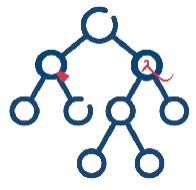
\includegraphics[height=1.0cm]{msca_logo.png}}%
    \end{center}

    \vspace{0.6cm}

    % Main title with Q logos on sides (with clickable links)
    \begin{center}
        \begin{minipage}{0.1\textwidth}
            \centering
            \href{https://quantlet.com}{
\includegraphics[height=1.1cm]{ql_logo.png}}
        \end{minipage}%
        \begin{minipage}{0.78\textwidth}
            \centering
            {\LARGE\bfseries\usebeamercolor[fg]{title}\inserttitle}

            \vspace{0.3cm}

            {\usebeamerfont{subtitle}\usebeamercolor[fg]{title}\insertsubtitle}
        \end{minipage}%
        \begin{minipage}{0.1\textwidth}
            \centering
            \href{https://quantinar.com}{
\includegraphics[height=1.1cm]{qr_logo.png}}
        \end{minipage}
    \end{center}

    \vspace{0.6cm}

    % Authors (left aligned)
    \hspace{0.5cm}{\usebeamerfont{author}\insertauthor}

    \vspace{0.3cm}

    % Institute/Affiliations (left aligned)
    \hspace{0.5cm}\begin{minipage}[t]{0.9\textwidth}
        \raggedright\small\insertinstitute
    \end{minipage}
}

%=============================================================================
% THEOREM ENVIRONMENTS
%=============================================================================
\theoremstyle{definition}
\setbeamertemplate{theorems}[numbered]
\ifdefined\tsalang
\newtheorem{defn}{Definiție}
\newtheorem{thm}{Teoremă}
\newtheorem{prop}{Propoziție}
\newtheorem{rmk}{Observație}
\else
\newtheorem{defn}{Definition}
\newtheorem{thm}{Theorem}
\newtheorem{prop}{Proposition}
\newtheorem{rmk}{Remark}
\fi

%=============================================================================
% CENTRED MINIPAGE (no extra vertical space)
%=============================================================================
\newenvironment{cminipage}[1]{%
    \par\noindent\hfill\begin{minipage}{#1}\ignorespaces
}{%
    \end{minipage}\hfill\null\par
}

%=============================================================================
% CUSTOM COMMANDS
%=============================================================================
\newcommand{\E}{\mathbb{E}}
\newcommand{\Var}{\text{Var}}
\newcommand{\Cov}{\text{Cov}}
\newcommand{\Corr}{\text{Corr}}
\newcommand{\R}{\mathbb{R}}
\newcommand{\N}{\mathbb{N}}
\newcommand{\Z}{\mathbb{Z}}
\newcommand{\B}{\mathbf{B}}
\newcommand{\imark}{\textcolor{MainBlue}{\textbullet}}
\newcommand{\RMSE}{\text{RMSE}}
\newcommand{\MAE}{\text{MAE}}
\newcommand{\MAPE}{\text{MAPE}}

% Boldface vector/matrix commands (VAR, VECM, state space; also used by the older TSA decks)
\newcommand{\bY}{\mathbf{Y}}
\newcommand{\bX}{\mathbf{X}}
\newcommand{\bA}{\mathbf{A}}
\newcommand{\bB}{\mathbf{B}}
\newcommand{\bepsilon}{\boldsymbol{\varepsilon}}
\newcommand{\bSigma}{\boldsymbol{\Sigma}}
\newcommand{\bPhi}{\boldsymbol{\Phi}}
\newcommand{\bGamma}{\boldsymbol{\Gamma}}
\newcommand{\bPi}{\boldsymbol{\Pi}}
\newcommand{\bc}{\mathbf{c}}
\newcommand{\balpha}{\boldsymbol{\alpha}}
\newcommand{\bbeta}{\boldsymbol{\beta}}
\newcommand{\bvarepsilon}{\boldsymbol{\varepsilon}}

% Legacy seminar marks (older TSA seminar decks)
\newcommand{\correct}{\textcolor{Forest}{\checkmark}}
\newcommand{\incorrect}{\textcolor{Crimson}{\texttimes}}


\newcommand{\qlurl}[1]{https://github.com/danpele/Time-Series-Analysis/tree/main/Quantlets/Ch_10/#1}
\renewcommand{\nb}{\colaburl{notebooks/EN/chapter10_seminar_notebook.ipynb}}
\renewcommand{\nbname}{chapter10\_seminar\_notebook.ipynb}
% left column: full width in the student version, narrower next to the solution
\newcommand{\taskw}{\ifsolutions 0.47\textwidth\else 0.96\textwidth\fi}
\newcommand{\solw}{\ifsolutions 0.49\textwidth\else 0pt\fi}

% Clickable citations (DOIs verified via Crossref)
\newcommand{\refHP}{\href{https://doi.org/10.1007/978-3-031-13584-2}{Huang and Petukhina (2022)}}
\newcommand{\refDK}{\href{https://doi.org/10.1093/acprof:oso/9780199641178.001.0001}{Durbin and Koopman (2012)}}
\newcommand{\refHarvey}{\href{https://doi.org/10.1017/CBO9781107049994}{Harvey (1989)}}
\newcommand{\refHamilton}{\href{https://doi.org/10.2307/j.ctv14jx6sm}{Hamilton (1994)}}
\newcommand{\refKN}{\href{https://doi.org/10.7551/mitpress/6444.001.0001}{Kim and Nelson (1999)}}
\newcommand{\refSS}{\href{https://doi.org/10.1007/978-3-319-52452-8}{Shumway and Stoffer (2017)}}
\newcommand{\refKalman}{\href{https://doi.org/10.1115/1.3662552}{Kalman (1960)}}
\newcommand{\refRTS}{\href{https://doi.org/10.2514/3.3166}{Rauch, Tung and Striebel (1965)}}
\newcommand{\refMuth}{\href{https://doi.org/10.1080/01621459.1960.10482064}{Muth (1960)}}
\newcommand{\refHKOS}{\href{https://doi.org/10.1007/978-3-540-71918-2}{Hyndman et al.\ (2008)}}
\newcommand{\refHJ}{\href{https://doi.org/10.1002/jae.3950080302}{Harvey and Jaeger (1993)}}
\newcommand{\refHPf}{\href{https://doi.org/10.2307/2953682}{Hodrick and Prescott (1997)}}
\newcommand{\refHamHP}{\href{https://doi.org/10.1162/rest\_a\_00706}{Hamilton (2018)}}
\newcommand{\refSW}{\href{https://doi.org/10.1086/654119}{Stock and Watson (1989)}}
\newcommand{\refGRS}{\href{https://doi.org/10.1016/j.jmoneco.2008.05.010}{Giannone, Reichlin and Small (2008)}}
\newcommand{\refHamMS}{\href{https://doi.org/10.2307/1912559}{Hamilton (1989)}}
\newcommand{\refHamEM}{\href{https://doi.org/10.1016/0304-4076(90)90093-9}{Hamilton (1990)}}
\newcommand{\refKim}{\href{https://doi.org/10.1016/0304-4076(94)90036-1}{Kim (1994)}}
\newcommand{\refCP}{\href{https://doi.org/10.1198/073500107000000296}{Chauvet and Piger (2008)}}
\newcommand{\refHSus}{\href{https://doi.org/10.1016/0304-4076(94)90067-1}{Hamilton and Susmel (1994)}}
\newcommand{\refLL}{\href{https://doi.org/10.1080/07350015.1990.10509794}{Lamoureux and Lastrapes (1990)}}
\newcommand{\refDI}{\href{https://doi.org/10.1016/S0304-4076(01)00073-2}{Diebold and Inoue (2001)}}

\title[Time Series Analysis]{Time Series Analysis}
\subtitle{Seminar 10: State space models, Kalman filter and Markov switching\ifsolutions\ (instructor version)\fi}
\author[D.T. Pele]{Daniel Traian PELE}
\institute{Bucharest University of Economic Studies\\
IDA Institute Digital Assets\\
Blockchain Research Center\\
AI4EFin Artificial Intelligence for Energy Finance\\
Romanian Academy, Institute for Economic Forecasting\\
MSCA Digital Finance}
\date{}

%=============================================================================
\providecommand{\tsaapplink}[3]{\hypertarget{#2}{}\hyperlink{#1}{\beamergotobutton{#3}}}  % APPLINKS-MACROS
\providecommand{\tsaappback}[2]{\begin{tikzpicture}[remember picture,overlay]\node[anchor=south east] at ([xshift=-3mm,yshift=7mm]current page.south east){\hyperlink{#1}{\beamerreturnbutton{#2}}};\end{tikzpicture}}  % APPLINKS-MACROS
\providecommand{\tsachlink}[2]{\href{#1}{#2}}  % APPLINKS-MACROS
\providecommand{\tsachlinkt}[2]{\href{#1}{\usebeamercolor[fg]{frametitle}#2}}  % APPLINKS-MACROS
\begin{document}
%=============================================================================

{
\setbeamertemplate{headline}{}
\setbeamertemplate{footline}{}
\begin{frame}[noframenumbering]
    \titlepage
\end{frame}
}
% BEGIN-ACRONYMS (generat de latex/acronyms.py; nu editati manual)
\begin{frame}{Acronyms used in this material}
\setbeamertemplate{itemize/enumerate body begin}{\tiny}
\begin{columns}[T]
\begin{column}{0.49\textwidth}
\begin{itemize}\setlength{\itemsep}{0pt}
    \item \textbf{AI}: Artificial Intelligence
    \item \textbf{AR}: AutoRegressive (model); in event studies: Abnormal Return
    \item \textbf{BET}: Bucharest Exchange Trading (index)
    \item \textbf{BIC}: Bayesian Information Criterion
    \item \textbf{CBO}: Congressional Budget Office
    \item \textbf{EODHD}: EOD Historical Data (market-data provider)
    \item \textbf{FRED}: Federal Reserve Economic Data
    \item \textbf{GARCH}: Generalised AutoRegressive Conditional Heteroskedasticity
    \item \textbf{GDP}: Gross Domestic Product
    \item \textbf{GDPC1}: Real Gross Domestic Product, chained dollars (FRED series code)
    \item \textbf{GDPPOT}: Real Potential Gross Domestic Product (FRED series code)
    \item \textbf{HICP}: Harmonised Index of Consumer Prices
    \item \textbf{HP}: Hodrick–Prescott (filter)
\end{itemize}
\end{column}
\begin{column}{0.49\textwidth}
\begin{itemize}\setlength{\itemsep}{0pt}
    \item \textbf{INDPRO}: Industrial Production Index (FRED series code)
    \item \textbf{NBER}: National Bureau of Economic Research
    \item \textbf{OLS}: Ordinary Least Squares
    \item \textbf{SD}: Standard Deviation
    \item \textbf{SE}: Standard Error
    \item \textbf{SES}: Simple Exponential Smoothing
    \item \textbf{UC}: Unobserved Components (model)
    \item \textbf{US}: United States
    \item \textbf{USREC}: US Recession indicator (FRED series code)
    \item \textbf{VAT}: Value Added Tax
\end{itemize}
\end{column}
\end{columns}
\end{frame}
% END-ACRONYMS

\begin{frame}{Today's question and route}
\itemsize{\small}
\begin{itemize}
    \item \textbf{Question}: how do we estimate a quantity we never observe (a level, a trend, a regime) from noisy data, one period at a time?
    \begin{itemize}
        \item this seminar comes \textbf{before} Lecture 10: the section ``What you need today'' gives every definition the tasks use
    \end{itemize}
    \item Route
    \begin{itemize}
        \item Part A: the Kalman filter by hand; exponential smoothing as a steady state; state space forms; durations; the Hamilton filter
        \item Part B: Romanian inflation; the US output gap; US industrial production and recessions; BET volatility regimes
        \item Part C: regimes of Romanian inflation since 1996; an AI answer to audit
    \end{itemize}
    \item Notebook for today: \href{\nb}{open the seminar notebook in Google Colab}; each task names its notebook section
\end{itemize}
\end{frame}

\begin{frame}{Exercise map}
\itemsize{\small}
\begin{center}
\footnotesize
\begin{tabular}{>{\raggedright\arraybackslash}p{1.1cm}>{\raggedright\arraybackslash}p{7.5cm}>{\raggedright\arraybackslash}p{1.9cm}>{\raggedright\arraybackslash}p{1.4cm}}
\toprule
\textbf{Task} & \textbf{Question} & \textbf{Type} & \textbf{Model} \\
\midrule
A1, A2 & the Kalman filter of a local level model for three periods; a missing value & Solved, Proposed & A1 \\
A3, A4 & steady state and exponential smoothing; state space forms and forecasts & Solved, Proposed & A3 \\
A5, A6 & durations of regimes; one step of the Hamilton filter & Solved, Proposed & A5 \\
B1, B2 & underlying Romanian inflation; the US output gap & Solved, Proposed & B1 \\
B3, B4 & recessions in US industrial production; BET volatility regimes & Solved, Proposed & B3 \\
C1, C2 & Romanian inflation regimes; what is wrong in an AI answer? & Proposed & B3, A1--A6 \\
\bottomrule
\end{tabular}
\end{center}
\begin{itemize}
    \item \textbf{[Solved]}: full solution in the slides and in the notebook, a model to follow; \textbf{[Proposed]}: you solve it, following the model
\end{itemize}
\end{frame}

\begin{frame}{Data used}
\itemsize{\small}
\begin{center}
\footnotesize
\begin{tabular}{llll}
\toprule
\textbf{Series} & \textbf{Source} & \textbf{Frequency} & \textbf{Period} \\
\midrule
HICP, Romania & Eurostat (prc\_hicp\_minr) & monthly, 2015 = 100 & 1996--2026 \\
real GDP and potential GDP, US & FRED (GDPC1, GDPPOT) & quarterly & 1947--2026 \\
industrial production, US & FRED (INDPRO) & monthly & 1960--2019 \\
NBER recession indicator & FRED (USREC) & monthly & 1960--2019 \\
BET, S\&P 500 & EODHD & weekly, from daily closes & 2000--2026 \\
\bottomrule
\end{tabular}
\end{center}
\begin{itemize}
    \item Monthly inflation: $100\Delta\ln P_t$, seasonally adjusted (SA) by removing the monthly means (\tsachlink{https://danpele.github.io/Time-Series-Analysis/EN/Courses/chapter4_seasonality_forecasting.pdf}{Chapter 4}); CBO output gap: $100(\mathrm{GDP}_t/\mathrm{GDPPOT}_t - 1)$
    \item In the notebook: \texttt{kalman\_by\_hand}, \texttt{local\_level\_ml}, \texttt{uc\_fit}, \texttt{hamilton\_filter}, \texttt{MarkovRegression}; no account or key is needed
\end{itemize}
\end{frame}


%=============================================================================
\section{What you need today}
%=============================================================================

\begin{frame}{What you need today (1/4): the state space form}
\itemsize{\small}
\begin{itemize}
    \item \textbf{State space form}: $y_t = Z\alpha_t + \varepsilon_t$ (measurement), $\alpha_{t+1} = T\alpha_t + R\eta_t$ (transition); $\varepsilon_t \sim N(0, H)$, $\eta_t \sim N(0, Q)$
    \begin{itemize}
        \item $\alpha_t$: the \textbf{state}, not observed; forecasts iterate the transition: $\hat\alpha_{T+h} = T^h\hat\alpha_T$
    \end{itemize}
    \item \textbf{Local level}: $y_t = \mu_t + \varepsilon_t$, $\mu_{t+1} = \mu_t + \eta_t$; signal-to-noise ratio $q = \sigma^2_\eta/\sigma^2_\varepsilon$
    \begin{itemize}
        \item \textbf{local linear trend}: $\mu_{t+1} = \mu_t + \beta_t + \eta_t$, $\beta_{t+1} = \beta_t + \zeta_t$; state $(\mu_t, \beta_t)'$
    \end{itemize}
    \item \textbf{AR(2)} in state space form: $\alpha_t = (y_t, y_{t-1})'$, $T = \begin{pmatrix}\phi_1 & \phi_2\\ 1 & 0\end{pmatrix}$, $Z = (1,\ 0)$, $H = 0$
    \begin{itemize}
        \item \textbf{simple exponential smoothing} (SES, \tsachlink{https://danpele.github.io/Time-Series-Analysis/EN/Courses/chapter0_introduction.pdf}{Chapter 0}): $\ell_t = \alpha y_t + (1-\alpha)\ell_{t-1}$, forecast $\hat y_{t+1} = \ell_t$
    \end{itemize}
\end{itemize}
\end{frame}

\begin{frame}{What you need today (2/4): the Kalman filter of the local level model}
\itemsize{\small}
\begin{itemize}
    \item Start with a prediction $a_t$ of $\mu_t$ and its variance $P_t$; when $y_t$ arrives \refKalman:
    \begin{itemize}
        \item $v_t = y_t - a_t$ (surprise), \quad $F_t = P_t + \sigma^2_\varepsilon$, \quad $K_t = P_t/F_t$ (\textbf{Kalman gain})
        \item update: $a_{t|t} = a_t + K_tv_t$, \quad $P_{t|t} = P_t(1 - K_t)$
        \item prediction: $a_{t+1} = a_{t|t}$, \quad $P_{t+1} = P_{t|t} + \sigma^2_\eta$
    \end{itemize}
    \item \textbf{Missing} $y_t$: no update, $a_{t|t} = a_t$, $P_{t|t} = P_t$; forecasts of every horizon equal $a_{n+1}$
    \begin{itemize}
        \item \textbf{steady state}: $\bar P = \sigma^2_\varepsilon(q + \sqrt{q^2 + 4q})/2$, $\bar K = \bar P/(\bar P + \sigma^2_\varepsilon)$; then $a_{t+1} = \bar Ky_t + (1 - \bar K)a_t$ is SES with $\alpha = \bar K$ \refMuth
        \item inverse map: $q = \alpha^2/(1 - \alpha)$
    \end{itemize}
\end{itemize}
\end{frame}

\begin{frame}{What you need today (3/4): likelihood, smoothing, trend and cycle}
\itemsize{\small}
\begin{itemize}
    \item \textbf{Likelihood} (prediction-error decomposition): $\log L = -\frac12\sum_t(\log 2\pi + \log F_t + v_t^2/F_t)$, maximised over the variances
    \begin{itemize}
        \item \textbf{filtered} $a_{t|t}$ uses $y_1..y_t$ (real time); \textbf{smoothed} $\hat\mu_t$ uses the whole sample (history) \refDK
    \end{itemize}
    \item \textbf{Output gap}: the cycle $\psi_t$ in $100\log\mathrm{GDP}_t = \mu_t + \psi_t$ (trend plus cycle)
    \begin{itemize}
        \item \textbf{UC model} \refHarvey: smooth trend ($\Delta^2\mu_{t+1} = \zeta_t$) plus an AR(2) cycle, estimated by the Kalman filter
        \item \textbf{HP filter} \refHPf: $\min\sum(y_t - \tau_t)^2 + 1600\sum(\Delta^2\tau_t)^2$, a two-sided smoother
        \item \textbf{Hamilton filter} \refHamHP: residual of OLS of $y_{t+8}$ on $1, y_t, \dots, y_{t-3}$
    \end{itemize}
\end{itemize}
\end{frame}

\begin{frame}{What you need today (4/4): Markov switching}
\itemsize{\small}
\begin{itemize}
    \item \textbf{Markov switching} \refHamMS: $y_t = \mu_{S_t} + \varepsilon_t$, $\varepsilon_t \sim N(0, \sigma^2_{S_t})$, regime $S_t \in \{1, 2\}$ follows a Markov chain
    \begin{itemize}
        \item $p_{ij} = \Pr(S_t = j \mid S_{t-1} = i)$; \textbf{expected duration} of regime $i$: $1/(1 - p_{ii})$
        \item \textbf{ergodic} probability $\pi_1 = (1 - p_{22})/(2 - p_{11} - p_{22})$; $h$-step transitions: $\mathbf{P}^h$
    \end{itemize}
    \item \textbf{Hamilton filter}: predict $\Pr(S_t = 1 \mid Y_{t-1}) = p_{11}\xi_{t-1} + (1 - p_{22})(1 - \xi_{t-1})$, with $\xi_{t-1} = \Pr(S_{t-1} = 1 \mid Y_{t-1})$
    \begin{itemize}
        \item update with the Normal densities $f_j(y_t)$: $\xi_t = \dfrac{\Pr(S_t = 1 \mid Y_{t-1})f_1(y_t)}{\Pr(S_t = 1 \mid Y_{t-1})f_1(y_t) + \Pr(S_t = 2 \mid Y_{t-1})f_2(y_t)}$
        \item \textbf{filtered} probabilities for real time, \textbf{smoothed} ones for history; \texttt{statsmodels}: \texttt{MarkovRegression}
    \end{itemize}
\end{itemize}
\end{frame}


%=============================================================================
\section{Part A: computations on paper}
%=============================================================================

\begin{frame}{A1: the Kalman filter for three periods [Solved]}
\itemsize{\scriptsize}
\begin{columns}[T]
\begin{column}{0.47\textwidth}
\begin{block}{Task}
\begin{itemize}
    \item Local level with $\sigma^2_\varepsilon = 1$, $\sigma^2_\eta = 1$; prior $a_1 = 0$, $P_1 = 1$; data $y = (1, 3, 2)$.
    \item 1. For $t = 1, 2, 3$ compute $F_t$, $K_t$, $v_t$, $a_{t|t}$, $P_{t|t}$ and the next prediction.
    \item 2. Give the forecast of $y_4$ and its variance.
    \item 3. Compute the steady-state gain $\bar K$ for $q = 1$.
    \item Report: a table of the three steps, one forecast, $\bar K$.
\end{itemize}
\end{block}
\end{column}
\begin{column}{0.49\textwidth}
\begin{exampleblock}{Solution}
\begin{itemize}
    \item 1. $t = 1$: $F = 2$, $K = 0.5$, $v = 1$, $a_{1|1} = 0.5$, $P_{1|1} = 0.5$; $a_2 = 0.5$, $P_2 = 1.5$
    \item $t = 2$: $F = 2.5$, $K = 0.6$, $v = 2.5$, $a_{2|2} = 0.5 + 0.6 \cdot 2.5 = 2$, $P_{2|2} = 0.6$; $a_3 = 2$, $P_3 = 1.6$
    \item $t = 3$: $F = 2.6$, $K = 0.615$, $v = 0$, $a_{3|3} = 2$, $P_{3|3} = 0.62$
    \item 2. $\hat y_4 = a_4 = 2.00$; $P_4 = 1.62$; $\Var = P_4 + \sigma^2_\varepsilon = 1.62 + 1$
    \item 3. $\bar P = (1 + \sqrt5)/2 = 1.618$ (the golden ratio), $\bar K = 0.618$; $K_t$ is already 0.615 at $t = 3$
\end{itemize}
\end{exampleblock}
\end{column}
\end{columns}
\end{frame}

\begin{frame}{A2: a missing observation [Proposed]}
\propsub
\itemsize{\scriptsize}
\begin{columns}[T]
\begin{column}{\taskw}
\begin{block}{Task}
\begin{itemize}
    \item Local level with $\sigma^2_\varepsilon = 2$, $\sigma^2_\eta = 0.5$; $a_1 = 5$, $P_1 = 2$; data $y = (6, \text{missing}, 4)$. Model: A1.
    \item 1. Run the filter for $t = 1, 2, 3$, skipping the update at $t = 2$.
    \item 2. Explain why $K_3$ equals $K_1$.
    \item 3. Compute $\bar K$ for this $q$ and the equivalent SES weight.
    \item Report: the three steps, one sentence, $\bar K$.
\end{itemize}
\end{block}
\end{column}
\begin{column}{\solw}
\solonly{%
\begin{exampleblock}{Solution}
\begin{itemize}
    \item 1. $t = 1$: $F = 4$, $K = 0.5$, $v = 1$, $a_{1|1} = 5.5$, $P_{1|1} = 1$; $a_2 = 5.5$, $P_2 = 1.5$
    \item $t = 2$: no update; $a_3 = 5.5$, $P_3 = 1.5 + 0.5 = 2$
    \item $t = 3$: $F = 4$, $K = 0.5$, $v = -1.5$, $a_{3|3} = 4.75$, $P_{3|3} = 1$; $a_4 = 4.75$, $P_4 = 1.50$
    \item 2. The missing year adds $\sigma^2_\eta$ without an update: $P_3 = P_1 = 2$, so the gain is the same; uncertainty that grows makes the next observation count more
    \item 3. $q = 0.25$: $\bar P = 1.281$, $\bar K = 0.390 = \alpha_{SES}$
\end{itemize}
\end{exampleblock}
}
\end{column}
\end{columns}
\end{frame}

\begin{frame}{A3: exponential smoothing is a steady-state Kalman filter [Solved]}
\itemsize{\scriptsize}
\begin{columns}[T]
\begin{column}{0.47\textwidth}
\begin{block}{Task}
\begin{itemize}
    \item A local level model and simple exponential smoothing (SES).
    \item 1. Show that the steady-state update $a_{t+1} = a_t + \bar K(y_t - a_t)$ is SES.
    \item 2. Compute $\bar K$ for $q = 1$ and $q = 0.25$.
    \item 3. An SES model has $\alpha = 0.3$. Find the $q$ of the local level model behind it.
    \item Report: one line of algebra, two gains, one $q$.
\end{itemize}
\end{block}
\end{column}
\begin{column}{0.49\textwidth}
\begin{exampleblock}{Solution}
\begin{itemize}
    \item 1. $a_{t+1} = \bar Ky_t + (1 - \bar K)a_t$: the SES recursion with $\alpha = \bar K$ and $\ell_t = a_{t+1}$
    \item 2. $q = 1$: $\bar P/\sigma^2_\varepsilon = (1 + \sqrt5)/2 = 1.618$, $\bar K = 1.618/(1.618 + 1) = 0.618$; $q = 0.25$: $\bar P/\sigma^2_\varepsilon = 0.640$, $\bar K = 0.390$
    \item 3. From $\bar P = \bar P(1 - \bar K) + \sigma^2_\eta$: $\sigma^2_\eta = \bar K\bar P$ and $\bar P = \alpha\sigma^2_\varepsilon/(1 - \alpha)$, so $q = \alpha^2/(1 - \alpha) = 0.09/0.7 = 0.129$
    \item a small $\alpha$ means a level that moves little relative to the noise
\end{itemize}
\end{exampleblock}
\end{column}
\end{columns}
\end{frame}

\begin{frame}{A4: state space forms and forecasts [Proposed]}
\propsub
\itemsize{\scriptsize}
\begin{columns}[T]
\begin{column}{\taskw}
\begin{block}{Task}
\begin{itemize}
    \item An AR(2) with $\phi_1 = 0.5$, $\phi_2 = 0.3$, $\sigma^2 = 1$; a local linear trend. Model: A1 (the prediction step).
    \item 1. Write $Z$, $T$, $R$, $Q$ and $H$ for the AR(2).
    \item 2. With the last state $(y_T, y_{T-1}) = (2, 1)$, compute the forecasts for $h = 1, 2, 3$ by $\hat\alpha_{T+h} = T\hat\alpha_{T+h-1}$.
    \item 3. Write $Z$ and $T$ of the local linear trend and forecast three steps from $\mu_T = 100$, $\beta_T = 2$.
    \item Report: two sets of matrices and six forecasts.
\end{itemize}
\end{block}
\end{column}
\begin{column}{\solw}
\solonly{%
\begin{exampleblock}{Solution}
\begin{itemize}
    \item 1. $Z = (1,\ 0)$, $T = \begin{pmatrix}0.5 & 0.3\\ 1 & 0\end{pmatrix}$, $R = (1,\ 0)'$, $Q = 1$, $H = 0$
    \item 2. $0.5 \cdot 2 + 0.3 \cdot 1 = 1.300$; $0.5 \cdot 1.300 + 0.3 \cdot 2 = 1.250$; $0.5 \cdot 1.250 + 0.3 \cdot 1.300 = 1.015$
    \item 3. $Z = (1,\ 0)$, $T = \begin{pmatrix}1 & 1\\ 0 & 1\end{pmatrix}$; forecasts 102, 104, 106: a straight line with slope $\beta_T$
\end{itemize}
\end{exampleblock}
}
\end{column}
\end{columns}
\end{frame}

\begin{frame}{A5: durations of recessions and expansions [Solved]}
\itemsize{\scriptsize}
\begin{columns}[T]
\begin{column}{0.47\textwidth}
\begin{block}{Task}
\begin{itemize}
    \item A two-regime model of GDP growth: regime 1 (recession) with $p_{11} = 0.75$, regime 2 (expansion) with $p_{22} = 0.95$.
    \item 1. Write the transition matrix and compute the expected durations.
    \item 2. Compute the ergodic probabilities.
    \item 3. Starting in a recession, compute the probability of a recession two quarters later.
    \item Report: two durations, two probabilities, one two-step probability.
\end{itemize}
\end{block}
\end{column}
\begin{column}{0.49\textwidth}
\begin{exampleblock}{Solution}
\begin{itemize}
    \item 1. $\mathbf{P} = \begin{pmatrix}0.75 & 0.25\\ 0.05 & 0.95\end{pmatrix}$; durations $1/0.25 = 4$ and $1/0.05 = 20$ quarters
    \item 2. $\pi_1 = 0.05/(0.25 + 0.05) = 0.167$, $\pi_2 = 0.833$: one quarter in six is a recession quarter
    \item 3. $p^{(2)}_{11} = 0.75^2 + 0.25 \cdot 0.05 = 0.575$; the chance of an expansion is $0.425$
    \item the geometric duration: many recessions are short, a few are long; the mean is 4 quarters
\end{itemize}
\end{exampleblock}
\end{column}
\end{columns}
\end{frame}

\begin{frame}{A6: one step of the Hamilton filter [Proposed]}
\propsub
\itemsize{\scriptsize}
\begin{columns}[T]
\begin{column}{\taskw}
\begin{block}{Task}
\begin{itemize}
    \item The model of A5 with $\mu_1 = -0.5$, $\mu_2 = 1$, $\sigma = 1$; last quarter $\Pr(S_{t-1} = 1 \mid Y_{t-1}) = 0.2$; this quarter $y_t = -1$. Model: A5.
    \item 1. Compute the predicted probability $\Pr(S_t = 1 \mid Y_{t-1})$.
    \item 2. Compute the densities $f_1(y_t)$, $f_2(y_t)$ (standard Normal $\phi(0.5) = 0.352$, $\phi(2) = 0.054$) and the filtered probability.
    \item 3. Give the likelihood contribution and the predicted probability for next quarter.
    \item Report: four probabilities and one log-density.
\end{itemize}
\end{block}
\end{column}
\begin{column}{\solw}
\solonly{%
\begin{exampleblock}{Solution}
\begin{itemize}
    \item 1. $0.75 \cdot 0.2 + 0.05 \cdot 0.8 = 0.190$
    \item 2. $f_1 = \phi(-0.5) = 0.352$, $f_2 = \phi(-2) = 0.054$; $\xi_t = 0.190 \cdot 0.352/0.111 = 0.605$
    \item 3. $p(y_t \mid Y_{t-1}) = 0.111$, $\log = \ensuremath{-}2.202$; next prediction $0.75 \cdot 0.605 + 0.05 \cdot (1 - 0.605) = 0.473$
    \item one bad quarter moves the recession probability from 0.19 to 0.60
\end{itemize}
\end{exampleblock}
}
\end{column}
\end{columns}
\end{frame}


%=============================================================================
\section{Part B: real data and interpretation}
%=============================================================================

\begin{frame}{B1: underlying Romanian inflation [Solved]}
\itemsize{\footnotesize}
\begin{itemize}
\item \textbf{Question}: how fast does the underlying level of Romanian inflation move, and which exponential smoothing weight does the data choose?
\item \textbf{Inputs}: monthly HICP inflation, seasonally adjusted, 2005--2026 ($T = 260$)
\item \textbf{Tasks}
\begin{enumerate}
    \item Fit the local level model by maximum likelihood and report $\hat\sigma^2_\varepsilon$, $\hat\sigma^2_\eta$ and $\hat q$.
    \item Compute the steady-state gain $\bar K$ and compare it with the SES weight estimated directly.
    \item Plot the filtered and smoothed level ($\times 12$, in \% per year) and report its peak and its last value.
    \item Interpretation: what does the size of $\hat q$ say about monthly inflation?
\end{enumerate}
\item \textbf{Report}: three variances, two weights, two levels, one sentence
\item Notebook: section B1
\end{itemize}
\end{frame}

\begin{frame}{B1: solution [Solved]}
\itemsize{\scriptsize}
\begin{center}
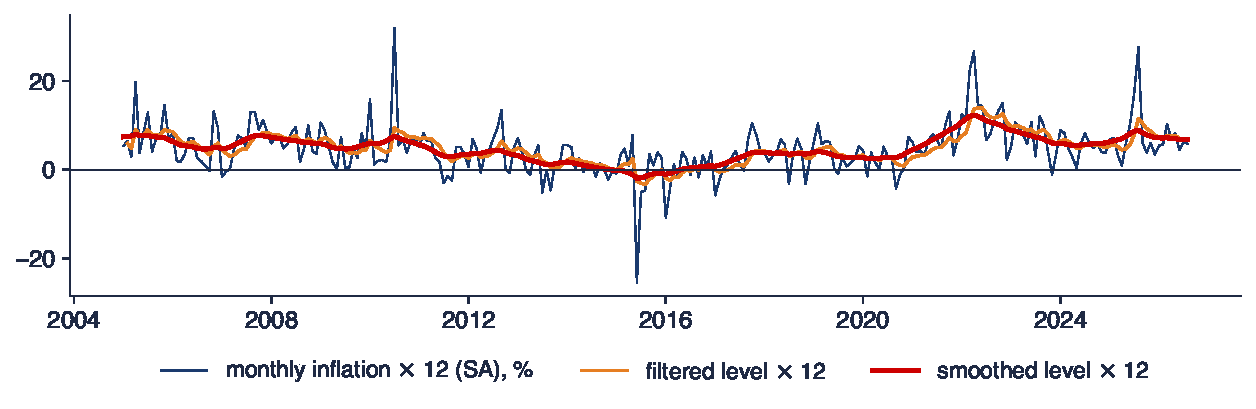
\includegraphics[width=0.96\textwidth,height=0.42\textheight,keepaspectratio]{ch10_sem_b1.pdf}
\end{center}
\vspace{-2mm}
\begin{itemize}
    \item $\hat\sigma^2_\varepsilon = 0.142$, $\hat\sigma^2_\eta = 0.0057$, $\hat q = 0.040$; $\bar K = 0.181$; SES by least squares: $\hat\alpha = 0.175$
    \item Smoothed level $\times 12$: peak 12.3\% (April 2022), low \ensuremath{-}2.0\% (June 2015), last 6.8\% (August 2026, SE 1.9); the raw series $\times 12$ has SD 5.6
    \item Interpretation: $q$ is small: most monthly movements are noise (tax changes, food and energy prices); each month moves the underlying level by about 0.181 of the surprise
\end{itemize}\quantlet{TSA\_ch10\_seminar}{\qlurl{TSA_ch10_seminar}}
\end{frame}

\begin{frame}{B2: the US output gap [Proposed]}
\itemsize{\footnotesize}
\begin{itemize}
\item \textbf{Question}: how close are three statistical output gaps to the official CBO gap, and which one would you use in real time?
\item \textbf{Inputs}: US real GDP and the CBO potential GDP, quarterly, 1949--2026; model: B1
\item \textbf{Tasks}
\begin{enumerate}
    \item Compute the UC cycle (smooth trend plus AR(2)), the HP gap ($\lambda = 1600$) and the Hamilton filter ($h = 8$, four lags) of $100\log\mathrm{GDP}$.
    \item Compute the CBO gap $100(\mathrm{GDP}/\mathrm{GDPPOT} - 1)$ and the correlation of each measure with it, including the filtered UC cycle.
    \item Report the standard deviations and the latest values.
    \item Interpretation: which measure would you use to judge the economy today?
\end{enumerate}
\item \textbf{Report}: five correlations, four standard deviations, four latest values, one sentence
\item Notebook: section B2
\end{itemize}
\end{frame}

\ifsolutions
\begin{frame}{B2: solution [Proposed]}
\itemsize{\scriptsize}
\begin{center}
\includegraphics[width=0.96\textwidth,height=0.42\textheight,keepaspectratio]{ch10_sem_b2.pdf}
\end{center}
\vspace{-2mm}
\begin{itemize}
    \item Correlation with the CBO gap: UC smoothed 0.77, UC filtered 0.88, HP 0.78, Hamilton 0.72; SD: CBO 2.3, UC 2.9, HP 1.6, Hamilton 3.3
    \item Latest: CBO 1.4\%, UC 0.7\%, HP \ensuremath{-}0.4\%, Hamilton 0.5\%
    \item Interpretation: the HP gap is the smallest and pulled to zero at the end of the sample; for today use a one-sided measure (filtered UC, Hamilton) and report its uncertainty
\end{itemize}\quantlet{TSA\_ch10\_seminar}{\qlurl{TSA_ch10_seminar}}
\end{frame}
\fi

\begin{frame}{B3: recessions in US industrial production [Solved]}
\itemsize{\footnotesize}
\begin{itemize}
\item \textbf{Question}: does a two-regime model of industrial production find the NBER recessions?
\item \textbf{Inputs}: monthly growth of US industrial production, 1960--2019 (93 NBER recession months)
\item \textbf{Tasks}
\begin{enumerate}
    \item Fit a two-regime model with switching mean and variance (\texttt{MarkovRegression}).
    \item Report the regime means and standard deviations, $p_{11}$, $p_{22}$ and the expected durations.
    \item Classify each month by the smoothed probability ($> 0.5$) and by the filtered probability, and compare with the NBER months.
    \item Interpretation: does the recession regime match the NBER recessions?
\end{enumerate}
\item \textbf{Report}: six parameters, two durations, two concordance tables, one sentence
\item Notebook: section B3
\end{itemize}
\end{frame}

\begin{frame}{B3: solution [Solved]}
\itemsize{\scriptsize}
\begin{center}
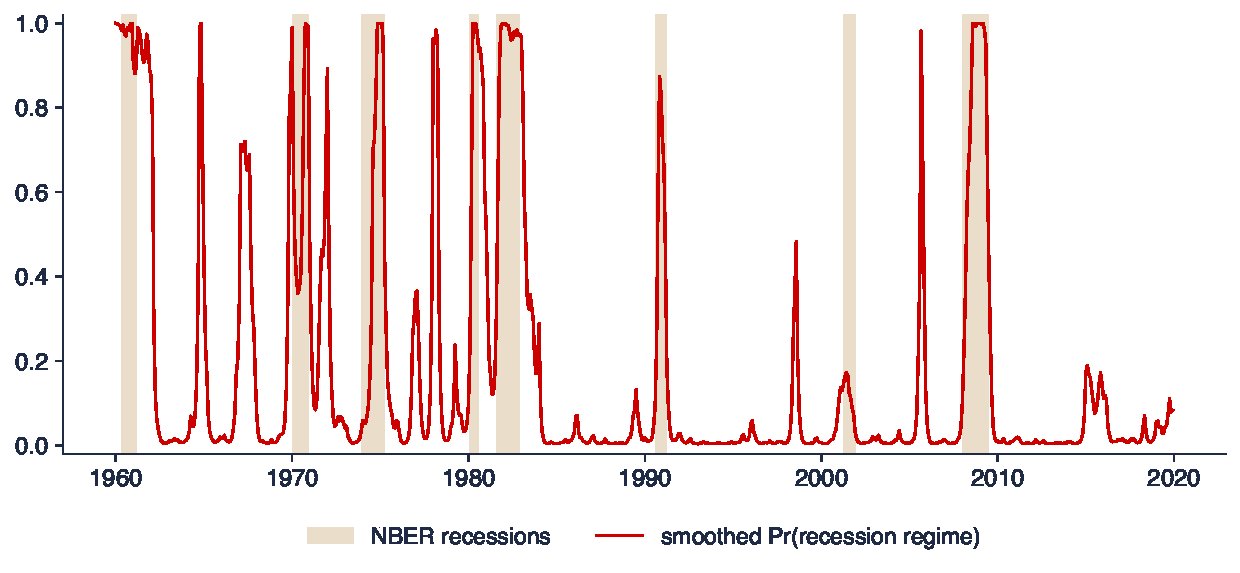
\includegraphics[width=0.96\textwidth,height=0.4\textheight,keepaspectratio]{ch10_sem_b3.pdf}
\end{center}
\vspace{-2mm}
\begin{itemize}
    \item Recession regime: mean \ensuremath{-}0.16\%, SD 1.30; expansion: mean 0.29\%, SD 0.51; $\hat p_{11} = 0.874$, $\hat p_{22} = 0.970$; durations 8.0 and 33.2 months; ergodic share 19\%
    \item Smoothed: 89\% of months agree, 69\% of NBER months found, 7\% false alarms; filtered: 86\%, 57\%, 10\%
    \item Interpretation: yes for the deep recessions; the regime is ``low and volatile growth'', so it also flags some slowdowns, and in real time it finds fewer recession months
\end{itemize}\quantlet{TSA\_ch10\_seminar}{\qlurl{TSA_ch10_seminar}}
\end{frame}

\begin{frame}{B4: volatility regimes of the BET [Proposed]}
\itemsize{\footnotesize}
\begin{itemize}
\item \textbf{Question}: does the Bucharest market have calm and turbulent regimes, and are they the same as those of the S\&P 500?
\item \textbf{Inputs}: weekly log returns of the BET and of the S\&P 500, 2000--2026; model: B3
\item \textbf{Tasks}
\begin{enumerate}
    \item Fit a two-regime model with switching mean and variance to BET returns; report the annualised volatilities and durations.
    \item List the three years with the largest share of turbulent weeks.
    \item Fit a GARCH(1,1) (\tsachlink{https://danpele.github.io/Time-Series-Analysis/EN/Courses/chapter5_conditional_volatility_garch.pdf}{Chapter 5}) and correlate its volatility with the regime-implied volatility.
    \item Interpretation: are the turbulent periods of the BET those of the S\&P 500?
\end{enumerate}
\item \textbf{Report}: two volatilities, two durations, three years, two correlations, one sentence
\item Notebook: section B4
\end{itemize}
\end{frame}

\ifsolutions
\begin{frame}{B4: solution [Proposed]}
\itemsize{\scriptsize}
\begin{center}
\includegraphics[width=0.96\textwidth,height=0.4\textheight,keepaspectratio]{ch10_sem_b4.pdf}
\end{center}
\vspace{-2mm}
\begin{itemize}
    \item Calm: 14\% per year, 33 weeks; turbulent: 40\% per year, 12 weeks; turbulent in 25\% of the weeks; years: 2009 (100\%), 2008 (94\%), 2001 (75\%)
    \item GARCH(1,1): $\alpha + \beta = 0.96$; correlation with the regime volatility 0.69; correlation of the turbulent probabilities of BET and S\&P 500: 0.48 (same classification in 78\% of the weeks)
    \item Interpretation: only partly: global crises (2008--2009) are common, but the BET has its own turbulent years (2001--2002) and was mostly calm in 2022 (27\% turbulent weeks, against 90\% for the S\&P 500)
\end{itemize}\quantlet{TSA\_ch10\_seminar}{\qlurl{TSA_ch10_seminar}}
\end{frame}
\fi


%=============================================================================
\section{Part C: open questions and AI critique}
%=============================================================================

\begin{frame}{C1: regimes of Romanian inflation [Proposed]}
\itemsize{\footnotesize}
\begin{itemize}
\item \textbf{Question}: how many inflation regimes has Romania had since 1996, and when did the low-inflation regime begin?
\item \textbf{Inputs}: monthly HICP inflation, not seasonally adjusted, 1996--2026; inflation targeting since August 2005; model: B3
\item \textbf{Tasks}
\begin{enumerate}
    \item Fit models with two and three regimes (switching mean and variance) and compare them by BIC.
    \item For three regimes, report the means, durations and the date when the low regime becomes permanent.
    \item Propose one more check (seasonality, a regime with an AR term, out-of-sample forecasts).
    \item Interpretation: did inflation targeting start the low-inflation regime?
\end{enumerate}
\item \textbf{Report}: six parameters, a date, a check and a project plan
\item Notebook: section C1
\end{itemize}
\end{frame}

\ifsolutions
\begin{frame}{C1: reference analysis [Proposed]}
\itemsize{\scriptsize}
\begin{center}
\includegraphics[width=0.96\textwidth,height=0.42\textheight,keepaspectratio]{ch10_sem_c1.pdf}
\end{center}
\vspace{-2mm}
\begin{itemize}
    \item Means (\% per month): low 0.40 (SD 0.41, about 4.8\% per year), medium 2.20, high 6.49; durations 40.1, 7.8, 4.3 months
    \item BIC: 910.8 with two regimes, 825.7 with three. The low regime appears in July 2002 and is the regime of almost every month from 2004, before inflation targeting; medium months return in 2010, 2022 and July--August 2025 (VAT increases in 2010 and 2025)
    \item Interpretation: disinflation started before 2005; targeting consolidated it. Project: add a regime-dependent AR term and compare forecasts with a local level model (B1)
\end{itemize}\quantlet{TSA\_ch10\_seminar}{\qlurl{TSA_ch10_seminar}}
\end{frame}
\fi

\begin{frame}{C2: audit an AI answer [Proposed]}
\itemsize{\scriptsize}
\begin{itemize}
    \item A student asked an AI assistant about state space and regime models. The answer:
    \item \aiprompt{(a) For the Nile, q = 0.097, so the equivalent exponential smoothing weight is alpha = q = 0.097.}
    \item \aiprompt{(b) The Kalman gain is K = sigma2\_eps / (P + sigma2\_eps): the noisier the data, the more weight they get.}
    \item \aiprompt{(c) With p11 = 0.75, recessions last p11 / (1 - p11) = 3 quarters on average.}
    \item \aiprompt{(d) To call a recession in real time, use smoothed\_marginal\_probabilities from statsmodels.}
    \item \aiprompt{(e) The last value of the HP gap is a reliable estimate of today's output gap.}
    \item \aiprompt{(f) In the local level model the forecasts of all horizons are equal; only their variance grows with the horizon.}
    \item Tasks
    \begin{itemize}
        \item 1. For each statement, say whether it is correct; if not, give the correct statement and, where possible, the correct number (Part A, notebook section C2).
        \item 2. Report: a list of six verdicts with one line of justification each.
    \end{itemize}
\end{itemize}
\end{frame}

\ifsolutions
\begin{frame}{C2: solution [Proposed]}
\itemsize{\scriptsize}
\begin{itemize}
    \item (a) Wrong: $\alpha = \bar K = 0.267$, not $q$; the map is $q = \alpha^2/(1 - \alpha)$ (A3)
    \item (b) Wrong: $K = P/(P + \sigma^2_\varepsilon)$; noisy data get \textbf{less} weight (A1)
    \item (c) Wrong: the expected duration is $1/(1 - p_{11}) = 4$ quarters (A5)
    \item (d) Wrong: smoothed probabilities use future data; in real time use \texttt{filtered\_marginal\_probabilities} (B3)
    \item (e) Wrong: HP is two-sided and its last values are revised when new quarters arrive \refHamHP; use a one-sided measure (B2)
    \item (f) Correct: $\hat y_{n+h} = a_{n+1}$ for all $h$, with variance $P_{n+1} + (h - 1)\sigma^2_\eta + \sigma^2_\varepsilon$
\end{itemize}\quantlet{TSA\_ch10\_seminar}{\qlurl{TSA_ch10_seminar}}
\end{frame}
\fi


%=============================================================================
\section{Wrap-up}
%=============================================================================

\begin{frame}{Key takeaways}
\itemsize{\small}
\begin{itemize}
    \item Kalman filter: $K_t = P_t/(P_t + \sigma^2_\varepsilon)$, $a_{t|t} = a_t + K_tv_t$; a missing value means no update
    \item Exponential smoothing is a local level filter in steady state: $\alpha = \bar K$, $q = \alpha^2/(1 - \alpha)$
    \item Romanian monthly inflation: small $q$, a slowly moving underlying level
    \item Markov switching: durations $1/(1 - p_{ii})$; filtered probabilities for real time, smoothed ones for history
    \item An AI answer is a draft: check the gain, the duration formula, filtered against smoothed
\end{itemize}
\end{frame}

\begin{frame}{After the seminar}
\itemsize{\small}
\begin{itemize}
    \item Lecture 10 develops each topic of today: the state space form, the filter and the smoother, the likelihood, trend and cycle, Markov switching
    \item Try the [Proposed] tasks in the notebook
    \item C1 can grow into a team project: inflation regimes in Romania and in the region
    \item Reading: \refDK, Ch.~2; \refHamMS; \refHamHP
    \item \textbf{The seminar is for practice and is not graded; the solutions of [Proposed] tasks are discussed in class}
\end{itemize}
\end{frame}


%=============================================================================
\section{References}
%=============================================================================

\begin{frame}{References}
\itemsize{\tiny}
\begin{itemize}
    \item Durbin, J., \& Koopman, S. J. (2012). \textit{Time Series Analysis by State Space Methods} (2nd ed.). Oxford University Press. \href{https://doi.org/10.1093/acprof:oso/9780199641178.001.0001}{doi:10.1093/acprof:oso/9780199641178.001.0001}
    \item Hamilton, J. D. (1989). A new approach to the economic analysis of nonstationary time series and the business cycle. \textit{Econometrica}, 57(2), 357--384. \href{https://doi.org/10.2307/1912559}{doi:10.2307/1912559}
    \item Hamilton, J. D. (2018). Why you should never use the Hodrick--Prescott filter. \textit{The Review of Economics and Statistics}, 100(5), 831--843. \href{https://doi.org/10.1162/rest\_a\_00706}{doi:10.1162/rest\_a\_00706}
    \item Harvey, A. C. (1989). \textit{Forecasting, Structural Time Series Models and the Kalman Filter}. Cambridge University Press. \href{https://doi.org/10.1017/CBO9781107049994}{doi:10.1017/CBO9781107049994}
    \item Hodrick, R. J., \& Prescott, E. C. (1997). Postwar U.S. business cycles: An empirical investigation. \textit{Journal of Money, Credit and Banking}, 29(1), 1--16. \href{https://doi.org/10.2307/2953682}{doi:10.2307/2953682}
    \item Kalman, R. E. (1960). A new approach to linear filtering and prediction problems. \textit{Journal of Basic Engineering}, 82(1), 35--45. \href{https://doi.org/10.1115/1.3662552}{doi:10.1115/1.3662552}
    \item Muth, J. F. (1960). Optimal properties of exponentially weighted forecasts. \textit{Journal of the American Statistical Association}, 55(290), 299--306. \href{https://doi.org/10.1080/01621459.1960.10482064}{doi:10.1080/01621459.1960.10482064}
\end{itemize}
\end{frame}

\end{document}
